%--------------------------------------
%ELECTROTECHNIQUE - SCHEMA DE LIAISON A LA TERRE
%--------------------------------------

%utiliser les environnement \begin{comment} \end{comment} pour mettre en commentaire le préambule une fois la programmation appelée dans le document maître (!ne pas oublier de mettre en commentaire \end{document}!)

\begin{comment}

\documentclass[a4paper, 11pt, twoside, fleqn]{memoir}

\usepackage{AOCDTF}

%--------------------------------------
%CANEVAS
%--------------------------------------

\newcommand\BoxColor{\ifcase\thechapshift blue!30\or brown!30\or pink!30\or cyan!30\or green!30\or teal!30\or purple!30\or red!30\or olive!30\or orange!30\or lime!30\or gray!\or magenta!30\else yellow!30\fi} %définition de la couleur des marqueurs de chapitre

\newcounter{chapshift} %compteur de chapitre du marqueur de chapitre
\addtocounter{chapshift}{-1}
	
\newif\ifFrame %instruction conditionnelle pour les couleurs des pages
\Frametrue

\pagestyle{plain}

% the main command; the mandatory argument sets the color of the vertical box
\newcommand\ChapFrame{%
\AddEverypageHook{%
\ifFrame
\ifthenelse{\isodd{\value{page}}}
  {\backgroundsetup{contents={%
  \begin{tikzpicture}[overlay,remember picture]
  \node[
  	rounded corners=3pt,
    fill=\BoxColor,
    inner sep=0pt,
    rectangle,
    text width=1.5cm,
    text height=5.5cm,
    align=center,
    anchor=north west
  ] 
  at ($ (current page.north west) + (-0cm,-2*\thechapshift cm) $) %nombre négatif = espacement des marqueurs entre les différents chapitres (à régler en fin de rédaction) (4.5cm vaut un espacement équivalement à la hauteur du marqueur, une page peut en contenir 6 avec cet espacement-la mais il est le plus équilibré)
    {\rotatebox{90}{\hspace*{.5cm}%
      \parbox[c][1.2cm][t]{5cm}{%
        \raggedright\textcolor{black}{\sffamily\textbf{\leftmark}}}}};
  \end{tikzpicture}}}
  }
  {\backgroundsetup{contents={%
  \begin{tikzpicture}[overlay,remember picture]
  \node[
  	rounded corners=3pt,
    fill=\BoxColor,
    inner sep=0pt,
    rectangle,
    text width=1.5cm,
    text height=5.5cm,
    align=center,
    anchor=north east
  ] 
  at ($ (current page.north east) + (-0cm,-2*\thechapshift cm) $) %nombre négatif = espacement des marqueurs entre les différents chapitres (à régler en fin de rédaction) (4.5cm vaut un espacement équivalement à la hauteur du marqueur, une page peut en contenir 6 avec cet espacement-la mais il est le plus équilibré)
    {\rotatebox{90}{\hspace*{.5cm}%
      \parbox[c][1.2cm][t]{5cm}{%
        \raggedright\textcolor{black}{\sffamily\textbf{\leftmark}}}}};
  \end{tikzpicture}}}%
  }
  \BgMaterial%
  \fi%
}%
  \stepcounter{chapshift}
}

\renewcommand\chaptermark[1]{\markboth{\thechapter.~#1}{}} %redéfinition du marqueur de chapitre pour ne contenir que le titre du chapitre %à personnaliser selon le nombre de chapitre dans le cours

%--------------------------------------
%corps du document
%--------------------------------------

\begin{document} %corps du document
	\openleft %début de chapitre à gauche

\end{comment}
\begin{figure}[H]
\caption{Câble en tranchée\label{fig:cable_tranchee}}
\tikzset{every picture/.style={line width=0.75pt}} %set default line width to 0.75pt        

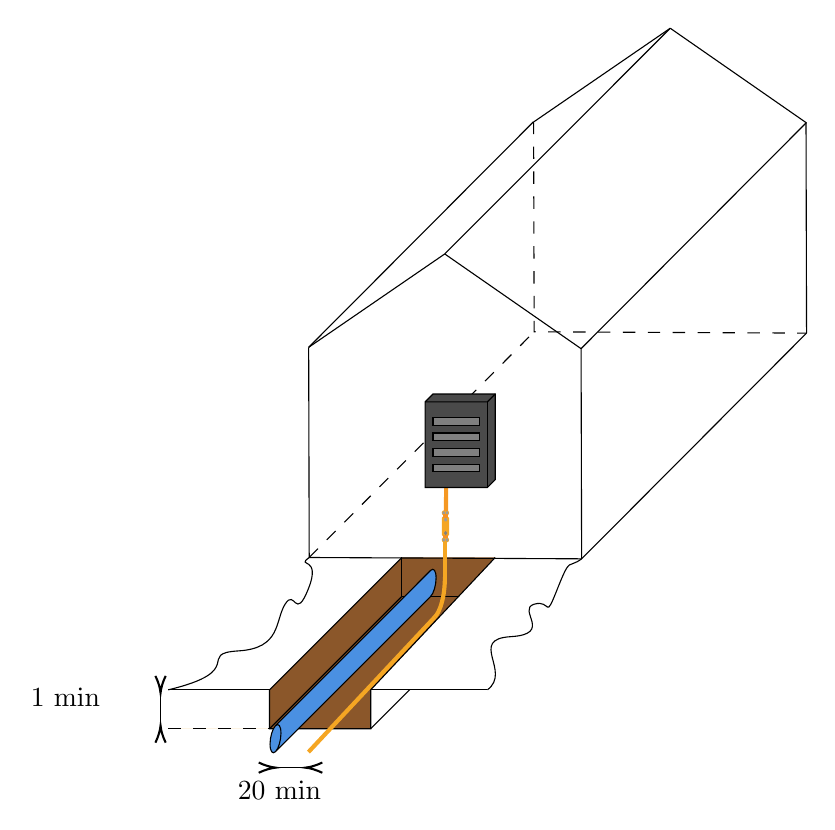
\begin{tikzpicture}[x=0.75pt,y=0.75pt,yscale=-0.75,xscale=0.75]
%uncomment if require: \path (0,751); %set diagram left start at 0, and has height of 751

%Straight Lines [id:da7829987710081011] 
\draw [fill={rgb, 255:red, 139; green, 87; blue, 42 }  ,fill opacity=1 ]   (280,340) -- (200,425) -- (200,450) -- (135,450) -- (135,425) -- (135,425) -- (220,340) ;
%Straight Lines [id:da49257416521092223] 
\draw    (220,365) -- (257,365) ;
%Straight Lines [id:da9081598274402687] 
\draw  [dash pattern={on 4.5pt off 4.5pt}]  (304.65,60) -- (305,195) -- (480,195.85) ;
%Straight Lines [id:da6348721638486958] 
\draw  [dash pattern={on 4.5pt off 4.5pt}]  (160.5,340) -- (305,195) ;
%Straight Lines [id:da1909522090160657] 
\draw    (160.15,205) -- (160.5,340) ;
%Straight Lines [id:da7207753640653374] 
\draw    (479.65,60.85) -- (480,195.85) ;
%Straight Lines [id:da6535753192189023] 
\draw    (160.15,205) -- (304.65,60) ;
%Straight Lines [id:da79950742566739] 
\draw    (247.57,145) -- (335.15,205.85) ;
%Straight Lines [id:da5547090580418039] 
\draw    (160.15,205) -- (247.57,145) ;
%Straight Lines [id:da920533856446613] 
\draw    (392.43,0) -- (480,60.85) ;
%Straight Lines [id:da11208478674638356] 
\draw    (305,60) -- (392.43,0) ;
%Straight Lines [id:da39788580291104303] 
\draw    (392.43,0) -- (247.57,145) ;
%Straight Lines [id:da7411479557367767] 
\draw    (479.65,60.85) -- (335.15,205.85) ;
%Straight Lines [id:da21547405248779972] 
\draw    (335.15,205.85) -- (335.5,340.85) ;
%Rounded Rect [id:dp28722339808467556] 
\draw  [color={rgb, 255:red, 245; green, 166; blue, 35 }  ,draw opacity=1 ][fill={rgb, 255:red, 245; green, 166; blue, 35 }  ,fill opacity=1 ] (246,311.33) .. controls (246,310.6) and (246.6,310) .. (247.33,310) -- (248.67,310) .. controls (249.4,310) and (250,310.6) .. (250,311.33) -- (250,311.33) .. controls (250,312.07) and (249.4,312.67) .. (248.67,312.67) -- (247.33,312.67) .. controls (246.6,312.67) and (246,312.07) .. (246,311.33) -- cycle ;
%Shape: Polygon [id:dp4090325935091489] 
\draw  [color={rgb, 255:red, 155; green, 155; blue, 155 }  ,draw opacity=1 ][fill={rgb, 255:red, 155; green, 155; blue, 155 }  ,fill opacity=1 ] (249.6,311.33) -- (249.35,311.91) -- (248.85,311.91) -- (248.6,311.33) -- (248.85,310.76) -- (249.35,310.76) -- cycle ;
%Shape: Polygon [id:dp35689183508447087] 
\draw  [color={rgb, 255:red, 155; green, 155; blue, 155 }  ,draw opacity=1 ][fill={rgb, 255:red, 155; green, 155; blue, 155 }  ,fill opacity=1 ] (247.4,311.33) -- (247.15,311.91) -- (246.65,311.91) -- (246.4,311.33) -- (246.65,310.76) -- (247.15,310.76) -- cycle ;

%Rounded Rect [id:dp06111128559002643] 
\draw  [color={rgb, 255:red, 245; green, 166; blue, 35 }  ,draw opacity=1 ][fill={rgb, 255:red, 245; green, 166; blue, 35 }  ,fill opacity=1 ] (246,328.67) .. controls (246,327.93) and (246.6,327.33) .. (247.33,327.33) -- (248.67,327.33) .. controls (249.4,327.33) and (250,327.93) .. (250,328.67) -- (250,328.67) .. controls (250,329.4) and (249.4,330) .. (248.67,330) -- (247.33,330) .. controls (246.6,330) and (246,329.4) .. (246,328.67) -- cycle ;
%Shape: Polygon [id:dp7859094987135327] 
\draw  [color={rgb, 255:red, 155; green, 155; blue, 155 }  ,draw opacity=1 ][fill={rgb, 255:red, 155; green, 155; blue, 155 }  ,fill opacity=1 ] (249.6,328.67) -- (249.35,329.24) -- (248.85,329.24) -- (248.6,328.67) -- (248.85,328.09) -- (249.35,328.09) -- cycle ;
%Shape: Polygon [id:dp0947001255145501] 
\draw  [color={rgb, 255:red, 155; green, 155; blue, 155 }  ,draw opacity=1 ][fill={rgb, 255:red, 155; green, 155; blue, 155 }  ,fill opacity=1 ] (247.4,328.67) -- (247.15,329.24) -- (246.65,329.24) -- (246.4,328.67) -- (246.65,328.09) -- (247.15,328.09) -- cycle ;

%Rounded Rect [id:dp5387904806018837] 
\draw  [color={rgb, 255:red, 245; green, 166; blue, 35 }  ,draw opacity=1 ][fill={rgb, 255:red, 245; green, 166; blue, 35 }  ,fill opacity=1 ] (246,314.73) .. controls (246,314.33) and (246.33,314) .. (246.73,314) -- (249.27,314) .. controls (249.67,314) and (250,314.33) .. (250,314.73) -- (250,325.27) .. controls (250,325.67) and (249.67,326) .. (249.27,326) -- (246.73,326) .. controls (246.33,326) and (246,325.67) .. (246,325.27) -- cycle ;
%Shape: Polygon [id:dp6617291355484505] 
\draw  [color={rgb, 255:red, 155; green, 155; blue, 155 }  ,draw opacity=1 ][fill={rgb, 255:red, 155; green, 155; blue, 155 }  ,fill opacity=1 ] (248.69,315.73) -- (248.4,316.39) -- (247.83,316.39) -- (247.54,315.73) -- (247.83,315.07) -- (248.4,315.07) -- cycle ;
%Shape: Rectangle [id:dp3731803592403742] 
\draw  [color={rgb, 255:red, 245; green, 145; blue, 35 }  ,draw opacity=1 ][fill={rgb, 255:red, 245; green, 145; blue, 35 }  ,fill opacity=1 ] (249,326) -- (247,326) -- (247,327.33) -- (249,327.33) -- cycle ;
%Shape: Rectangle [id:dp13543640418430414] 
\draw  [color={rgb, 255:red, 245; green, 145; blue, 35 }  ,draw opacity=1 ][fill={rgb, 255:red, 245; green, 145; blue, 35 }  ,fill opacity=1 ] (249,312.67) -- (247,312.67) -- (247,314) -- (249,314) -- cycle ;
%Shape: Ellipse [id:dp009996283185936261] 
\draw  [color={rgb, 255:red, 128; green, 128; blue, 128 }  ,draw opacity=1 ][fill={rgb, 255:red, 128; green, 128; blue, 128 }  ,fill opacity=1 ] (248.8,324.33) .. controls (248.8,323.85) and (248.51,323.47) .. (248.15,323.47) .. controls (247.79,323.47) and (247.5,323.85) .. (247.5,324.33) .. controls (247.5,324.81) and (247.79,325.2) .. (248.15,325.2) .. controls (248.51,325.2) and (248.8,324.81) .. (248.8,324.33) -- cycle ;

%Straight Lines [id:da07044954250685276] 
\draw [color={rgb, 255:red, 245; green, 152; blue, 35 }  ,draw opacity=1 ][line width=1.5]    (248.49,294.84) -- (248.33,310) ;
%Shape: Cube [id:dp8957361009096318] 
\draw  [fill={rgb, 255:red, 74; green, 74; blue, 74 }  ,fill opacity=1 ] (235,240) -- (240,235) -- (280,235) -- (280,290) -- (275,295) -- (235,295) -- cycle ; \draw   (280,235) -- (275,240) -- (235,240) ; \draw   (275,240) -- (275,295) ;
%Shape: Rectangle [id:dp22048605405624178] 
\draw  [fill={rgb, 255:red, 128; green, 128; blue, 128 }  ,fill opacity=1 ] (240,280) -- (270,280) -- (270,285) -- (240,285) -- cycle ;
%Shape: Rectangle [id:dp38722589110484673] 
\draw  [fill={rgb, 255:red, 128; green, 128; blue, 128 }  ,fill opacity=1 ] (240,270) -- (270,270) -- (270,275) -- (240,275) -- cycle ;
%Shape: Rectangle [id:dp6742075818101974] 
\draw  [fill={rgb, 255:red, 128; green, 128; blue, 128 }  ,fill opacity=1 ] (240,260) -- (270,260) -- (270,265) -- (240,265) -- cycle ;
%Shape: Rectangle [id:dp8945073743205151] 
\draw  [fill={rgb, 255:red, 128; green, 128; blue, 128 }  ,fill opacity=1 ] (240,250) -- (270,250) -- (270,255) -- (240,255) -- cycle ;
%Shape: Arc [id:dp4869608729068412] 
\draw  [draw opacity=0][line width=1.5]  (247.67,352.54) .. controls (247.66,364.36) and (244.94,374.42) .. (241.14,378.3) -- (237.67,352.5) -- cycle ; \draw  [color={rgb, 255:red, 245; green, 166; blue, 35 }  ,draw opacity=1 ][line width=1.5]  (247.67,352.54) .. controls (247.66,364.36) and (244.94,374.42) .. (241.14,378.3) ;
%Straight Lines [id:da9150475387692276] 
\draw [color={rgb, 255:red, 245; green, 166; blue, 35 }  ,draw opacity=1 ][line width=1.5]    (160,465) -- (241.14,378.3) ;
%Straight Lines [id:da2033450004552232] 
\draw [fill={rgb, 255:red, 245; green, 166; blue, 35 }  ,fill opacity=1 ]   (70,425) -- (135,425) ;
%Straight Lines [id:da7151214616154821] 
\draw    (200,425) -- (275,425) ;
%Curve Lines [id:da6063582718063134] 
\draw    (70,425) .. controls (121.5,412.67) and (87.4,401.64) .. (115,400) .. controls (142.6,398.36) and (138.42,380.61) .. (145,370) .. controls (151.58,359.39) and (151.4,381.64) .. (160,360) .. controls (168.6,338.36) and (151.6,346.68) .. (160.5,340) ;
%Curve Lines [id:da7510759130219333] 
\draw    (275,425) .. controls (290.74,413.2) and (262.4,392.49) .. (290,390.85) .. controls (317.6,389.22) and (293.6,373.36) .. (305,370) .. controls (316.4,366.64) and (311.4,381.64) .. (320,360) .. controls (328.6,338.36) and (326.6,347.53) .. (335.5,340.85) ;
%Straight Lines [id:da3682420377901341] 
\draw    (480,195.85) -- (335.5,340.85) ;
%Straight Lines [id:da9913786842235923] 
\draw    (220,365) -- (135,450) ;
%Straight Lines [id:da8269394900324805] 
\draw    (200,450) -- (225,425) ;
%Straight Lines [id:da9808722000068587] 
\draw    (220,340) -- (220,365) ;
%Straight Lines [id:da3541321557731596] 
\draw    (160.5,340) -- (335.5,340.85) ;
%Straight Lines [id:da5783336689263071] 
\draw    (65,427) -- (65,448) ;
\draw [shift={(65,448)}, rotate = 90] [color={rgb, 255:red, 0; green, 0; blue, 0 }  ][line width=0.75]    (10.93,-3.29) .. controls (6.95,-1.4) and (3.31,-0.3) .. (0,0) .. controls (3.31,0.3) and (6.95,1.4) .. (10.93,3.29)   ;
\draw [shift={(65,427)}, rotate = 270] [color={rgb, 255:red, 0; green, 0; blue, 0 }  ][line width=0.75]    (10.93,-3.29) .. controls (6.95,-1.4) and (3.31,-0.3) .. (0,0) .. controls (3.31,0.3) and (6.95,1.4) .. (10.93,3.29)   ;
%Straight Lines [id:da7565418229148708] 
\draw [color={rgb, 255:red, 245; green, 166; blue, 35 }  ,draw opacity=1 ][line width=1.5]    (247.67,330) -- (247.67,352.54) ;
%Shape: Can [id:dp7267813341154139] 
\draw  [fill={rgb, 255:red, 74; green, 144; blue, 226 }  ,fill opacity=1 ] (138.85,448.03) -- (238.5,348.28) .. controls (240.44,346.34) and (242.01,348.51) .. (242.01,353.13) .. controls (242.01,357.74) and (240.44,363.06) .. (238.5,365) -- (138.85,464.75) .. controls (136.91,466.69) and (135.34,464.52) .. (135.34,459.9) .. controls (135.34,455.29) and (136.91,449.97) .. (138.85,448.03) .. controls (140.79,446.09) and (142.36,448.26) .. (142.36,452.88) .. controls (142.36,457.5) and (140.79,462.81) .. (138.85,464.75) ;
%Straight Lines [id:da42695123304320515] 
\draw    (158,475) -- (139,475) ;
\draw [shift={(139,475)}, rotate = 180] [color={rgb, 255:red, 0; green, 0; blue, 0 }  ][line width=0.75]    (10.93,-3.29) .. controls (6.95,-1.4) and (3.31,-0.3) .. (0,0) .. controls (3.31,0.3) and (6.95,1.4) .. (10.93,3.29)   ;
\draw [shift={(158,475)}, rotate = 360] [color={rgb, 255:red, 0; green, 0; blue, 0 }  ][line width=0.75]    (10.93,-3.29) .. controls (6.95,-1.4) and (3.31,-0.3) .. (0,0) .. controls (3.31,0.3) and (6.95,1.4) .. (10.93,3.29)   ;
%Straight Lines [id:da04967441192853961] 
\draw [fill={rgb, 255:red, 245; green, 166; blue, 35 }  ,fill opacity=1 ] [dash pattern={on 4.5pt off 4.5pt}]  (70,450) -- (135,450) ;

% Text Node
\draw (-20,422) node [anchor=north west][inner sep=0.75pt]   [align=left] {\SI{1}{\meter} min};
% Text Node
\draw (113,482) node [anchor=north west][inner sep=0.75pt]   [align=left] {\SI{20}{\centi\meter} min};


\end{tikzpicture}

\end{figure}

%\end{document}

